\documentclass{article}
\usepackage{amsmath}
\usepackage{graphicx}
\newcommand{\system}[1]{\mathcal{Z}\{#1\}}

\begin{document}
\title{Discrete Assignment}
\author{Karyampudi Meghana Sai\\ EE23BTECH11031}
\maketitle

\section*{Problem Statement}
Write the first five terms of the sequence \(a_n = \frac{n(n^2+5)}{4}\).

\section*{Solution}
The relation between \(x(n)\) and \(u(n)\):
\begin{align}
 x(n) &= \left(\frac{(n+1)^3+5(n+1)}{4}\right) u(n)\label{eq:1}
\end{align}
Z-transform of \(n^ku(k)\) in terms of the \(k\)-th derivative of \(U(z)\):
\begin{align}
n^k u(n) &\overset{\text{ZT}}{\longleftrightarrow} (-1)^k z^k \frac{d^k}{dz^k}U(z)
\end{align}

\begin{align}
    \system{nu(n)} &= \frac{z^{-1}}{(1 - z^{-1})^2} \label{eq:3} \text{ [ROC: } \lvert z \rvert > 1\text{]} \\
    \system{n^2u(n)} &= \frac{(z^{-1})(1+z^{-1})}{(1 - z^{-1})^3} \label{eq:4} \text{ [ROC: } \lvert z \rvert > 1\text{]} \\
    \system{n^3u(n)} &= \frac{(z^{-1})(1+4z^{-1}+z^{-2})}{(1 - z^{-1})^4} \label{eq:5} \text{ [ROC: } \lvert z \rvert > 1\text{]}
\end{align}
Referencing the equations \eqref{eq:3}, \eqref{eq:4}, and \eqref{eq:5}.
\begin{align}
    \mathcal{X}(z) &= \frac{(z^{-1})(1+4z^{-1}+z^{-2})}{4(1-z^{-1})^4} + \frac{3(z^{-1})(1+z^{-1})}{4(1-z^{-1})^3} + \frac{2z^{-1}}{(1 - z^{-1})^2} + \frac{3}{2(1- z^{-1})} \\
    \mathcal{X}(z) &= \frac{3}{2(1-z^{-1})^3} + \frac{3z^{-2}}{2(1-z^{-1})^4}
\end{align}

\newpage
\begin{figure}
    \centering
    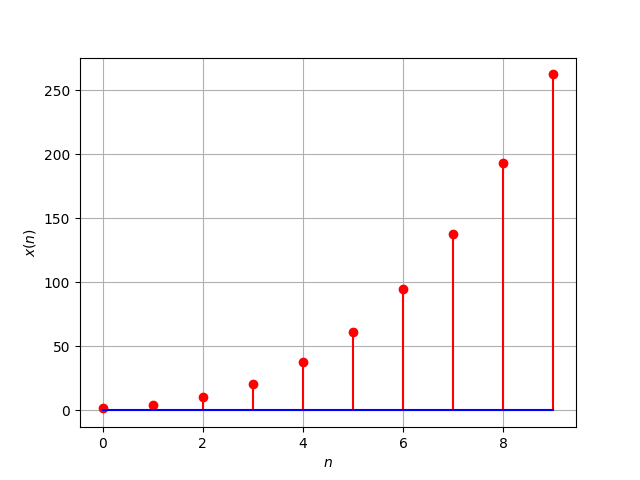
\includegraphics{figs/plot.png}
    \label{fig:your_label}
\end{figure}
\end{document}

